%!TEX root = root.tex

\chapter{Comprehensive discovery of driver genes and mutations in cancer}
\label{chap:ch7}
\chaptermark{Comprehensive driver discovery}

Over the past decade, The Cancer Genome Atlas (TCGA) has coordinated a monumental enterprise of data generation and genomic investigation across 33 cancer types, and numerous notable findings have emerged from this project (\url{https://cancergenome.nih.gov/publications}). The individual TCGA projects also motivated the development of many bioinformatic algorithms oriented toward discovery, characterization, and prioritization of cellular processes driving cancer based on pathways \cite{RN180}, genes \cite{RN49}, or individual variations \cite{RN181}. However, despite this remarkable progress, algorithms do not entirely agree on certain candidate cancer driver genes and mutations, necessitating continued expert curation to filter likely false positive findings. Moreover, previous PanCancer analyses \cite{RN96} have been limited to fewer cancer types and have largely avoided nominating rare driver mutations. 

\section{Mutational data set}
Mutation calls were produced by the Multi-Center Mutation Calling in Multiple Cancers (MC3) working group by harmonizing results of 7 algorithms \cite{RN167}. To reduce the false positive rate for driver gene discovery I implemented three strategies addressing known issues affecting driver detection and data quality (see Mutation calling quality control). The driver detection dataset ultimately consisted of 9,079 samples having 1,457,702 total mutations, where the number of mutations per sample was widely distributed across cancer types and was consistent with previous publications \cite{RN12, RN13, RN96}.

\subsection{Mutation calling quality control}
A publicly available MAF file (\url{https://synapse.org/MC3}) was recently compiled by the MC3 Working Group and is annotated with filter flags to highlight potential artifacts or discrepancies. This dataset represents the most uniform attempt to systematically provide mutation calls for TCGA tumors. The MC3 effort provided consensus calls from 7 software packages \cite{RN167}. Flagged artifacts include: non-exonic regions, whole-genome amplified (WGA) samples, exclusion lists, blood/tumor derived pairs, strand-bias, contamination estimations, oxo-guanine artifacts, low normal read depth, polymorphisms common in EXAC \cite{RN168}, mutations present in a panel of normal samples, non-preferred tumor normal pairs, and mutations outside the regions of interest for any caller. If a mutation was not assigned any flag and was called by 2 or more variant calling software packages, it received a 'PASS' identifier. I restricted our analysis to PASS calls with the exception of samples from OV and LAML, which were some of the earliest sequenced by TCGA. Preparations for these samples utilized whole genome amplified (WGA) DNA, an important factor in that the WGA process can induce artefactual mutations. Of the 412 OV and 141 LAML samples present in our data 347 (84\%) and 141 (100\%), respectively, had variants derived from WGA DNA. In order to maintain sample sizes and uniformity in mutation calling, I did not filter mutations containing only 'wga' filter tags from these two cancer types. I recognize multiple limitations of this mutation call set including the lack of structural variants and copy number alterations, as well as variability in sequencing depth and tumor purity. The above limitations may lead to variability in mutation detection; however, the MC3 dataset reflects the state-of-the-art in consensus mutation detection.

I also excluded highly mutated samples. These hypermutators were defined as samples with a mutation count exceeding Tukey's outlier condition, i.e. greater than 1.5 times the interquartile range above the third quartile in their respective cancer types (3Q + 1.5*IQR). Designation as a hypermutator also required the number of mutations in a sample to exceed 1000, a heuristic that limited the number of discarded samples in low mutation rate cancer types. LUAD, SKCM, and UCEC had hypermutator thresholds greater than 1000 mutations (1047, 2122, and 2545 respectively). I also excluded samples that were flagged by the analysis-working group based on pathology, but allowed \q{RNA degradation} samples to remain, as this factor is not particularly relevant for most driver prediction tools based on mutations. The final driver-discovery dataset consisted of 9,079 samples having a total of 791,637 missense mutations, 323,884 silent mutations, 96,196 3'UTR mutations, 57,900 nonsense mutations, 42,251 intronic mutations, 42,251 Frame shift deletions, 34,266 5' UTR, 21,804 splice site mutations, 19,856 RNA mutations, 11,305 frame shift insertions, 7,622 3' flanking mutations, 6,419 5' flanking mutations, 6,144 in-frame deletions, 1,362 translation start site mutations, 964 nonstop mutations, and 632 in-frame insertions.

\section{Driver gene discovery approach}
Using multiple tools can overcome numerous technical issues that confound individual statistical analyses to find driver genes, such as heterogeneous mutation rate across the genome \cite{RN13}, inflated significance for long genes \cite{RN169}, and false positive calls in cancers with high mutation rates \cite{RN70}. In the first phase, 8 different tools comprising algorithms based on mutation frequency (MuSiC2 \cite{RN43} and MutSig2CV \cite{RN14}), features (20/20+ \cite{RN70}, CompositeDriver(in preparation) and OncodriveFML \cite{RN86}), clustering (OncodriveCLUST \cite{RN54}), and externally defined regions (e-Driver \cite{RN153} and ActiveDriver \cite{RN98}) were used (\autoref{fig:driver_gene_approach}A). Each tool reported gene or mutation level scores and/or p-values along with a brief description of recommended cutoff thresholds or filters.

\begin{figure}[b!]
  \centering
  \makeatletter
  \let\@currsize\normalsize
  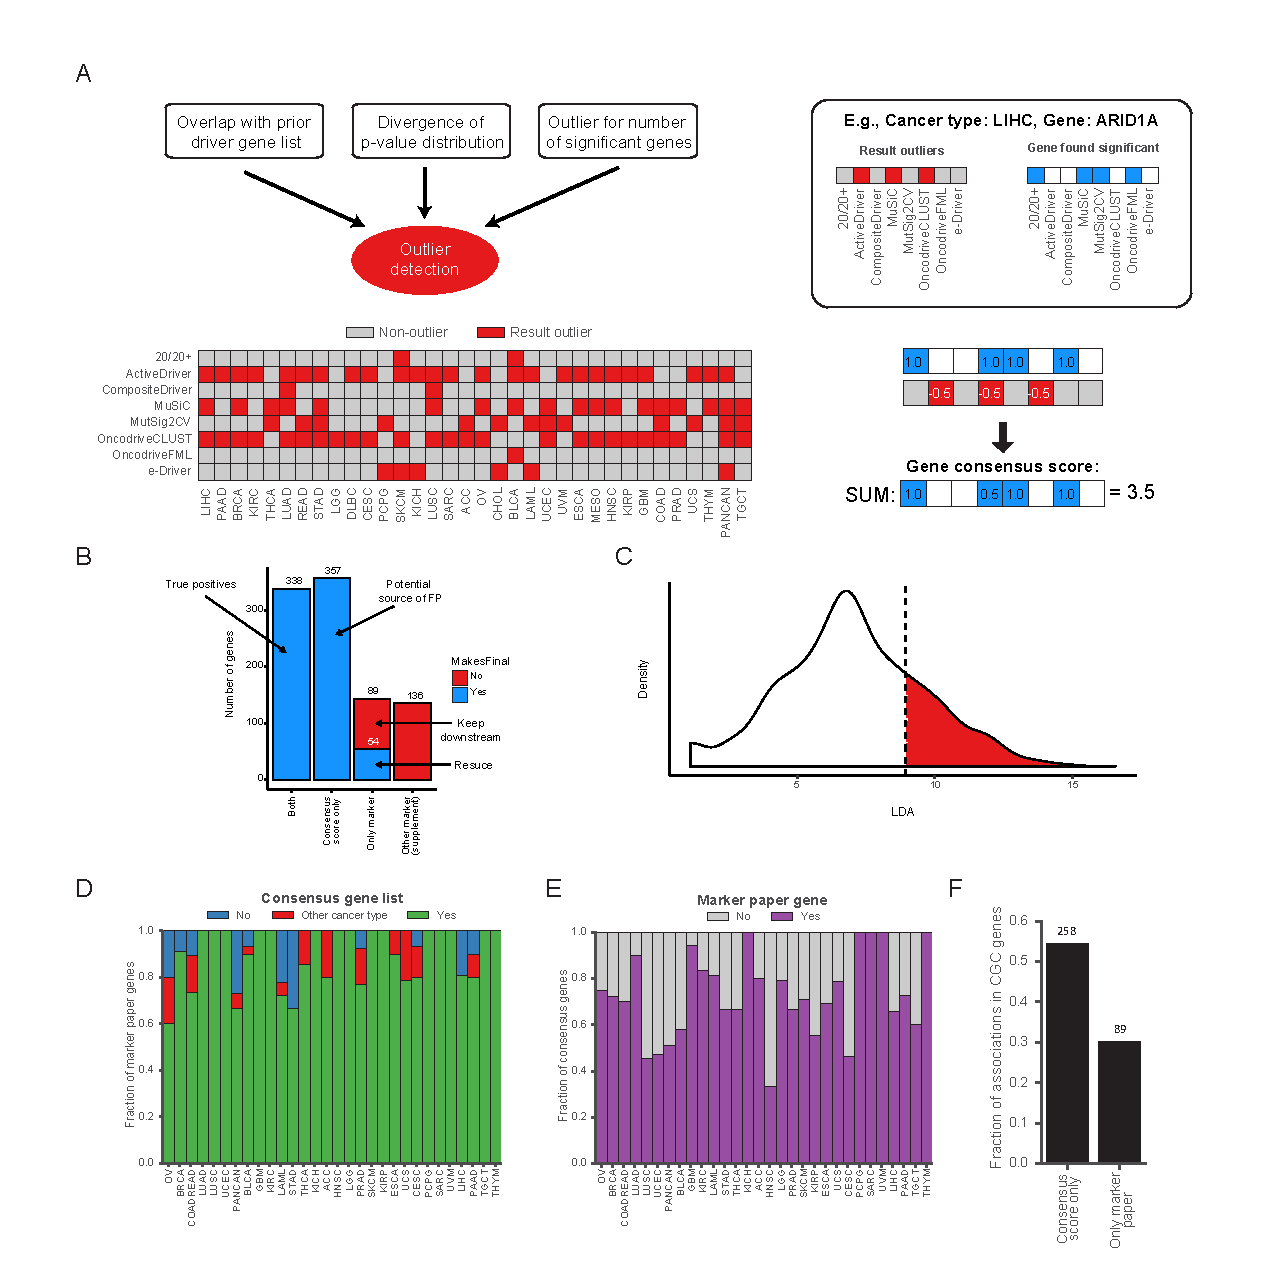
\includegraphics[width=\linewidth]{figures/chapter7/driver_gene_approach.pdf}
  \caption[Consensus Gene scores and SMG filtering.]{(Caption next page.)}
  \label{fig:driver_gene_approach}
\end{figure}
\addtocounter{figure}{-1}
\begin{figure} [t!]
  \caption[(continued) Consensus Gene scores and SMG filtering.]{(Figure previous page) Consensus Gene scores and SMG filtering. (A) Left, outlier detection was performed on a per analysis and method basis. Outliers were marked (red) based on the quasi-majority of three criteria: (1) low concordance with known cancer genes from Vogelstein et al (lower than median); (2) high divergence of p-value distribution from theoretical expectation (higher than median); and (3) abnormally high number of significant genes ($>$1.5x the interquartile range above the third quartile). The first two criteria were assessed based on the other tools within a single analysis, while the third criterion was assessed based on the same tool's results over all the individual cancer types (excluding the PanCancer analysis). Right, example calculation of the gene consensus score for ARID1A in the cancer type LIHC. A result from an outlier is down weighted, receiving a weight of 0.5 instead of 1.0. The gene consensus score is the sum of weights for tools finding that gene as significant. (B) Overlap of consensus gene list with prior TCGA marker papers. (C) Likely false positives were detected with a high Linear Discriminant Analysis (LDA) score threshold representing 90\% sensitivity for keeping associations found in Cancer Gene Census genes. LDA was trained to distinguish common false positives in exome sequencing from previous TCGA PanCancer marker papers. The LDA threshold was only applied to the potential source of false positive genes. (D) Fraction of marker paper genes highlighted in the main text that were also found in our consensus gene list. (E) Fraction of our consensus gene list found in previous TCGA marker papers.  (F) Fraction of associations found in the Cancer Gene Census (CGC) that were either found only in the consensus gene list or TCGA marker paper. }
\end{figure}

\subsection{Consensus methodology}
I identified a preliminary total of 2,101 potential drivers by taking the union of genes predicted by the eight driver-gene discovery tools.  As illustrated in \autoref{fig:driver_gene_approach}A, the increased number of false positive genes is likely due to any individual tool's capability to maintain sound statistical properties that handle a complex set of factors such as tumor heterogeneity, increased mutation rates, and variable sample sizes. I refined this list by calculating, for each gene predicted in each cancer type, a consensus score that compensated for outlier results and correlation among tools (\autoref{fig:driver_gene_approach}). The consensus score was defined as a weighted sum of the number of tools that predicted the gene to be a driver in each cancer type (see \autoref{sec:weighting}). I required a minimum of two tools to agree, where both could not be outliers (score$\geq$1.5). Although it is difficult to distinguish the overall performance improvement on a small number of held out CGC genes (\autoref{fig:gene_characteristics}A), the weighting strategy did have higher specificity (p=4.3e-8, McNemar test), which is preferable given concerns of false positives. Regardless, the consensus score performance on identifying CGC genes (\autoref{fig:gene_characteristics}A) support previous reports that merging the results from different algorithms improve cancer driver discovery \cite{RN96}. 

\begin{figure}
  \centering
  \makeatletter
  \let\@currsize\normalsize
  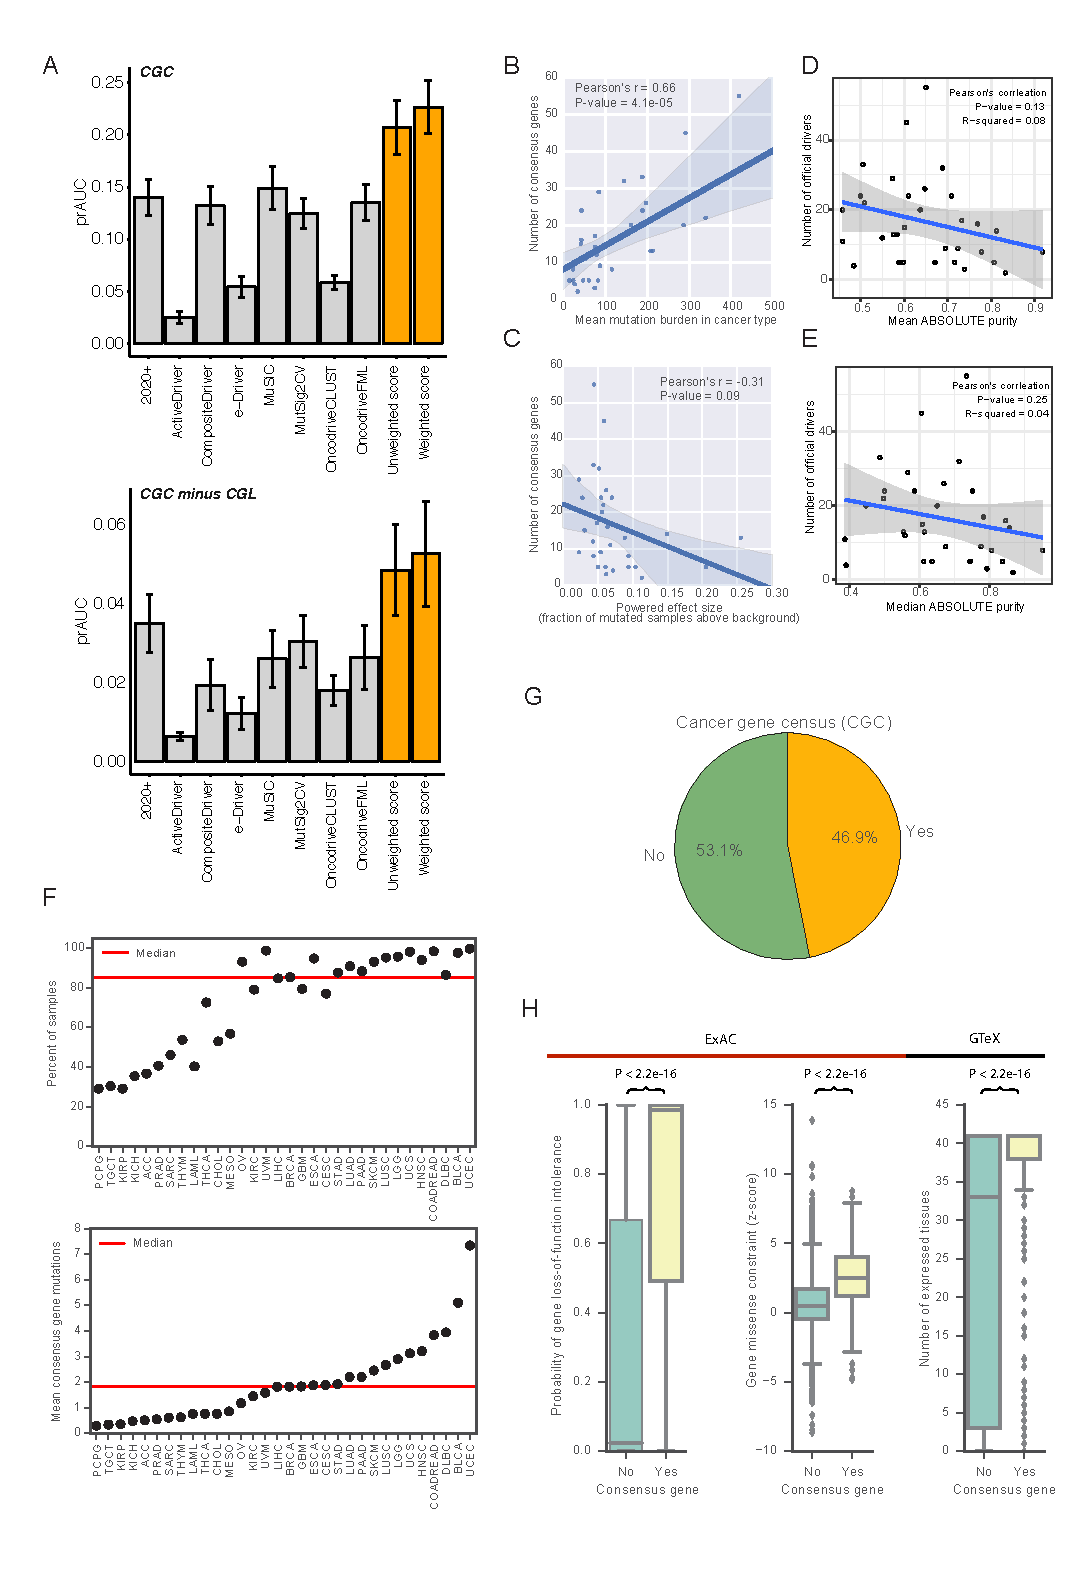
\includegraphics[width=0.9\linewidth]{figures/chapter7/analysis_of_cancer_driver_genes.pdf}
  \caption[Characteristics of consensus genes.]{(Caption next page.)}
  \label{fig:gene_characteristics}
\end{figure}
\addtocounter{figure}{-1}
\begin{figure} [t!]
\caption[(continued) Characteristics of consensus genes.]{(Figure previous page) Characteristics of consensus genes. (A) Predictive power of each individual driver gene detection method (in gray) and of the weighted and weighted scores (in orange). The predictive power was measured as prAUC, using all the genes in the Cancer Gene Census and a set that additionally excludes Cancer Genome Landscape genes used in outlier detection. Error bars, calculated by bootstrapping, indicate one standard deviation. (B) The number of consensus genes in each cancer type positively correlated with the average mutation burden. Shaded area indicates 95\% bootstrapped confidence interval. (C) Given the variability in powered effect size (fraction of mutated samples above background with 90\% power) in this study, there is a negative but not significant correlation with the number of consensus genes in each cancer type. COAD and READ were excluded because analysis was performed separately, but the final consensus genes were merged. (D) Pearson correlation between the number driver genes identified and median purity was calculated and plotted. (E) Pearson correlation between the number driver genes identified and mean purity was calculated and plotted. Summary statistics for p-value and r-squared value are reported in the top right corner of panels D and E. (F) Percent of samples containing a non-silent mutation stratified by cancer type. The red line indicates the median across cancer types (left) and average number of non-silent mutations in consensus genes per sample (right). (G) A pie chart showing the percent of consensus genes which are found in the Cancer Gene Census with annotations for small somatic mutations (missense, splice site, indel, and nonsense) (H) Consensus genes showed a higher probability for loss-of-function intolerance and missense mutation constraint of germline mutations based on ExAC, and were expressed (RPKM$>$1) in a wider number of tissues from GTeX (version 6). Given the high correlation of gene expression in the 11 brain regions assessed from GTEx, we took the median of multiple brain tissues, as done in Lek et al., 2016.}
\end{figure}

To maximize the coverage of our analysis and ensure the accuracy of our final list, previous findings were reviewed in 31 individual cancer types and PanCancer-12 from TCGA. For cancer types not yet having a TCGA publication, the relevant analysis working groups were consulted (LIHC, TGCT, UVM, SARC, PAAD, and THYM). I included in our final consensus list all those genes that were previously described as drivers by experts in the cancer-specific analysis of TCGA datasets and were also identified by at least one of the eight algorithms, even if they did not meet our consensus score threshold ($\geq$1.5)(\autoref{fig:gene_discovery}A). This resulted in an additional 54 gene-cancer pairs, such as ATR, CHEK2, IDH2, and ERCC2 in the PanCancer dataset and FOXA1 in BLCA, HRAS in SKCM, and MET in LUAD (\autoref{fig:driver_gene_approach}B-F). The majority of this effort resulted in linking cancer genes identified by our strategy to additional cancer types based on previous literature (32/54).  

\begin{figure}
  \centering
  \makeatletter
  \let\@currsize\normalsize
  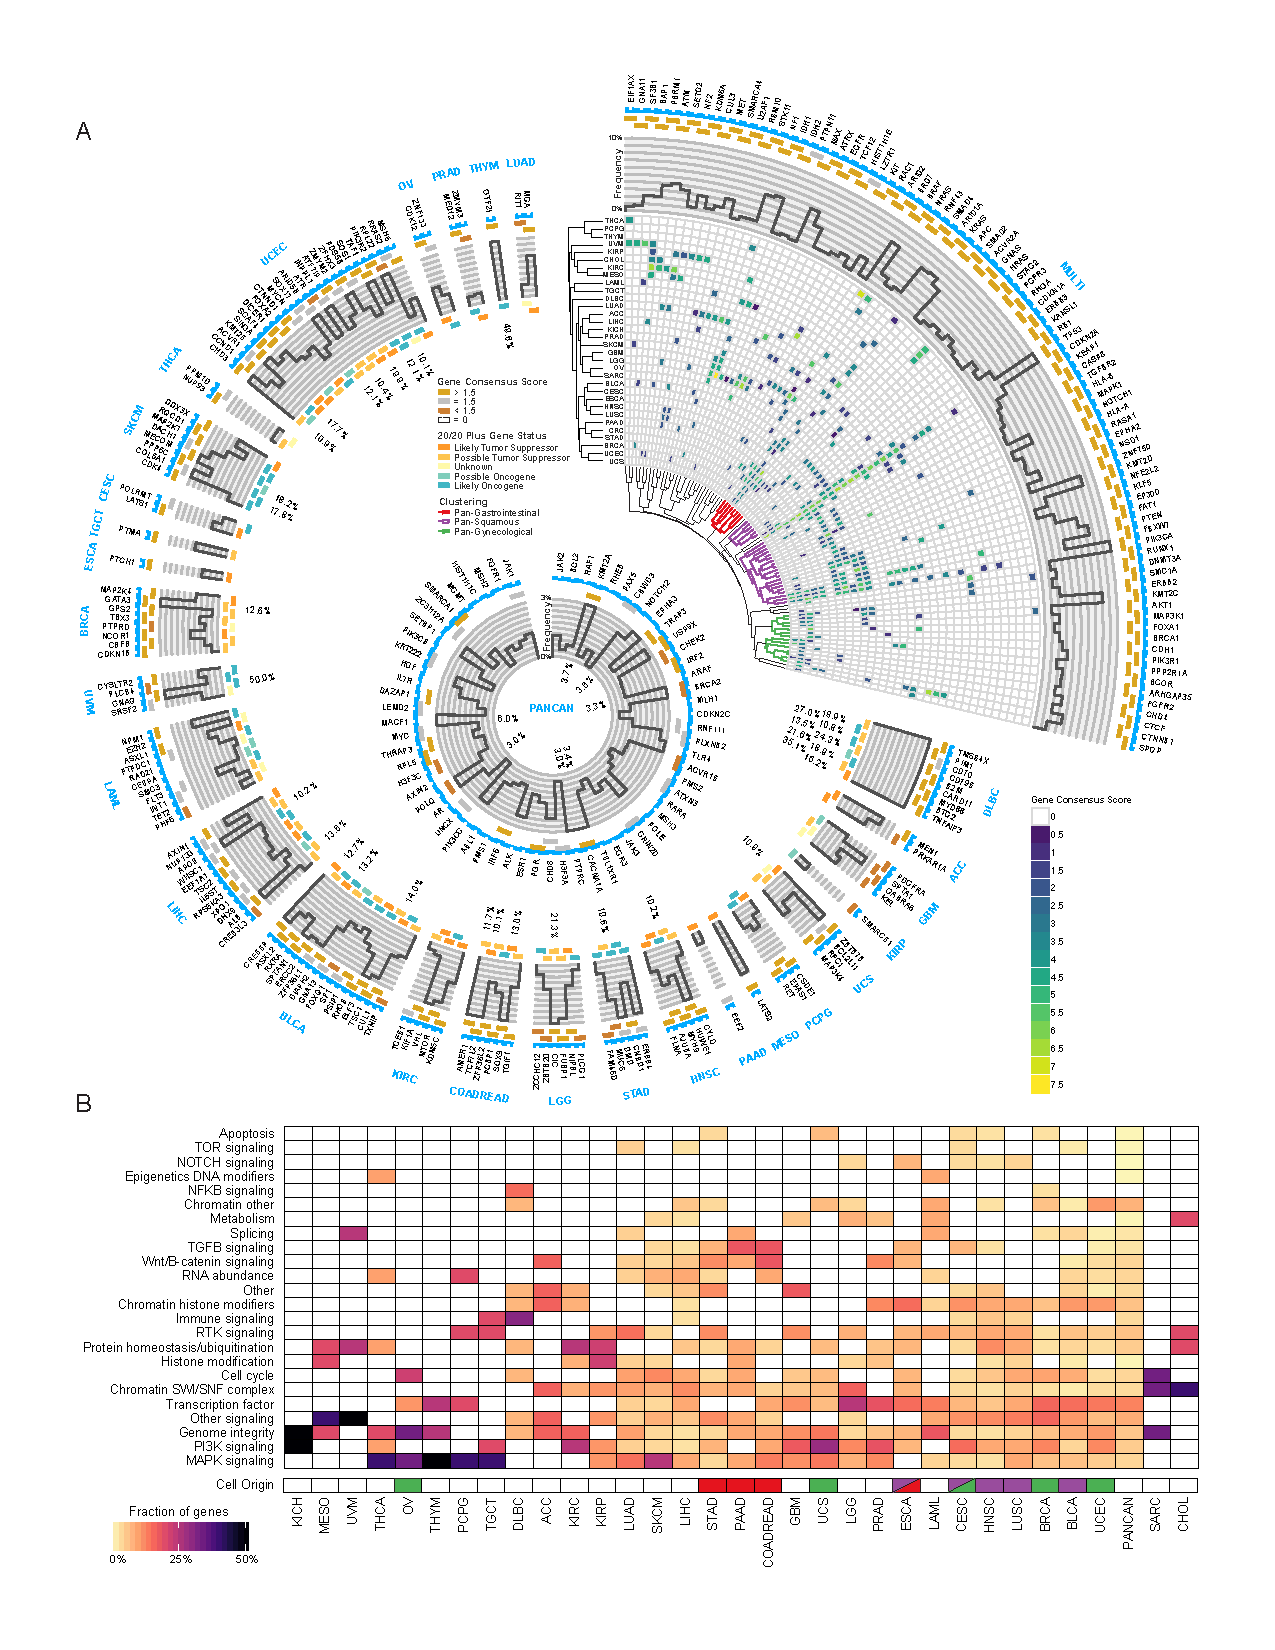
\includegraphics[width=\linewidth]{figures/chapter7/cancer_driver_genes.pdf}
  \caption[Cancer driver gene discovery]{(Caption next page.)}
  \label{fig:gene_discovery}
\end{figure}
\addtocounter{figure}{-1}
\begin{figure} [t!]
  \caption[(continued) Cancer driver gene discovery]{(Figure previous page) Cancer driver gene discovery: (A) Circos \cite{RN182} plot displays 299 cancer genes. Each sector indicates a unique cancer type (text in blue) with predicted drivers unique to that cancer type listed (gene name in black). Only tissues with at least one unique driver gene are shown. The top right sector shows all genes found significant in multiple cancer types. Next, a categorical score of gold, silver, or bronze is assigned to each gene based on the highest consensus score. If a gene was not scored and required rescue then the field is empty. The next ring illustrates the mutation frequency of a gene in our dataset. For the top right wedge, the PanCancer frequency is used, while cancer-type-specific frequencies are used in the remaining sectors. Where frequencies exceed the y-axis limit of 10\%, the innermost label indicates the frequency. The final ring uses a 5-point scale from orange to teal to represent each gene from likely tumor suppressor to likely oncogene, respectively, by the 20/20+ algorithm. Finally, in the top right slice we show hierarchical clustering of the gene consensus scores for genes that were found in more than one cancer type (note: CRC refers to the COADREAD cancer type). Additionally, significant gene clusters (permutation test) identified Pan-Gastrointestinal (red), Pan-Squamous (purple), and Pan-Gynecological tissues (green). The middle ring illustrates all genes that were only found using PanCancer results, or were otherwise rescued. (B) Heatmap showing clustering of different cancer types by pathway / biological process affected by associated consensus driver genes. Cell of origin for pan-gynecological, pan-gastrointestinal, and pan-squamous are colored as above.}
\end{figure}

To limit false positives in the expanded list, linear discriminant analysis was applied (\autoref{fig:driver_gene_approach}C). 45 genes were identified and removed from the consensus as they are likely false positives. These included CACNA1E in PanCancer, COL11A1 in LUAD, DST in GBM, and TTN in SKCM. The consensus list from the above systematic approach consisted of 258 unique genes. The average number of non-silent mutations per sample in our consensus gene list varied substantially by cancer type ranging from <1 in 12 cancer types (ACC, CHOL, KICH, KIRP, LAML, MESO, PCPG, PRAD, SARC, TGCT, THCA, and THYM) to 7.3 in UCEC. A median of 85\% of tumors harbored non-silent mutations in consensus genes across cancer types (\autoref{fig:gene_characteristics}F). 

Given the limitations of a systematic approach, 41 genes were manually rescued. In the rescue attempt, I started with a list of genes identified from previous TCGA marker papers but not found from our systematic approach. Genes were rescued with supportive evidence from the following sources: hypermutator phenotype related genes (since we excluded hypermutated samples in our systematic discovery; 6 genes), established cancer genes from LAML because of low quality variant calling originating from liquid tumor contamination of the normal samples (6 genes), genes supported by omic network tools (DriverNet and OncoIMPACT; 25 genes), and a gene supported by all three approaches from the driver mutation discovery (1 gene). Addition of genes to the final list was subjected to expert manual curation (3 genes). 

The final consensus gene list consisted of 299 unique genes across 33 cancer types and the PanCancer dataset (\autoref{fig:gene_discovery}A). The list captures most previously described driver genes for the majority of cancer types. I overlapped the cancer driver genes obtained from the consensus approach without manual curation with those from 5 independent studies in 4 cancer types (BRCA, PRAD, PAAD, and LIHC) of which one is whole-genome sequencing. The consensus approach always had a greater inter-study overlap, with an average increase of 26\% over only using a single tool, either MuSiC2 or MutSig2CV \cite{RN57, RN176, RN175, RN172, RN173, RN174}. Among the 299 genes, 59 novel genes were not previously identified in 6 previous PanCancer publications \cite{RN57, RN14, RN178, RN25, RN96, RN177, RN1} or the cancer gene census list (\url{http://cancer.sanger.ac.uk/census/})\cite{RN97}.

\subsection{Weighting strategy}
\label{sec:weighting}
Tools predicting cancer genes were weighted according to their performance in each cancer type, receiving half the weight if a result was deemed an outlier, thereby obligating additional tool agreement. Specifically, I examined quality metrics across tools and within the same tool, which allowed us to identify outlier results. I marked outliers based on the quasi-majority of three criteria: low concordance with known cancer genes, high divergence of p-value distribution from theoretical expectation, and abnormally high number of significant genes. The first criterion evaluated the fraction overlap of significant genes with a previously manually curated set of driver genes from \cite{RN25} compared with the median across all tools. The second criterion examined whether the divergence of observed p-values from those theoretically expected by the Mean Log Fold Change (MLFC) \cite{RN70} was greater than the median of all tools, which may indicate a tool's statistical assumptions may not be well satisfied. The third criterion examined whether a tool's prediction for particular cancer types appeared as an outlier in terms of the number of significant genes compared against all of the results for that tool (Tukey's outlier criterion: number significant $>$ 3Q + 1.5*IQR). I calculated a gene consensus score by summing the tools that declared the gene as being significant, with a weight of 1 for non-outlier results and 0.5 for outlier results.

\section{The landscape of cancer driver genes}

The final consensus list consists of 299 unique genes: 258 genes obtained from a systematic approach and 41 additional genes recovered after manual curation of previous TCGA marker papers with the majority (26 out of 41, 63\%) supported by additional -omic network tools (DriverNet and OncoIMPACT) not used in original SMG detection. Note that, for the rest of the analyses presented here, I will focus on the 258 genes set, but I acknowledge the limitations of a systematic approach by including the 41 genes rescued by manual curation in our final list to achieve comprehensiveness.

The list recovers most of the previously described driver genes for the majority of cancer types. In fact, in 20 out the 31 cancer types included in our study that had either been previously published or for which I had an internal list of known cancer driver genes, the recovery rate is 80\% or higher (\autoref{fig:driver_gene_approach}D and \autoref{fig:driver_gene_approach}E). The most significant outliers are STAD and the previous PanCancer study, for which I only recovered around 70\% of the previously described genes (\autoref{fig:driver_gene_approach}D). The consensus list also includes 59 novel genes that had not been described previously and other known drivers not previously associated with a given tissue. Predictions of known cancer driver genes in new tissues include ATRX in ACC, KMT2C, CTNNB1 and PTEN in BLCA, and ARID1A and KRAS in BRCA. Entirely novel predictions include GNA13 in BLCA (a homologue of the known drivers GNAQ and GNA11), RRAS2 in UCEC (with shared homology in KRAS and HRAS), and KIF1A in HNSC (a kinesin of the same family of the cancer driver KIF5B). 

The number of detected cancer driver genes varies among cancer types, with KICH having the fewest (2 genes) and UCEC having the most (55 genes). Furthermore, the ratio of predicted tumor suppressor genes and oncogenes vary widely by tissue (\autoref{fig:og_tsg_balance}). I observed a significant positive correlation (Pearson R=0.66, P value=4.1e-5) between the average mutation burden in a cancer type and the number of identified consensus genes (\autoref{fig:gene_characteristics}B). Study-based calculations for powered effect size in each cancer type did not entirely explain this phenomenon (Pearson R=-0.31, P value=0.09) (\autoref{fig:gene_characteristics}C). Regarding the associations of driver genes with different cancer types, many genes (142 out of 258) are associated with a single cancer, whereas 87 genes have driver roles in two or more cancer types, with an additional 29 genes uniquely identified using all samples combined-PanCancer approaches. As expected, TP53 is the most extreme case, as it is associated with 27 cancer types, followed by PIK3CA, KRAS, PTEN and ARID1A, each of which is associated with 15 or more tissue types (\autoref{fig:gene_discovery}A).

\begin{figure}
  \centering
  \makeatletter
  \let\@currsize\normalsize
  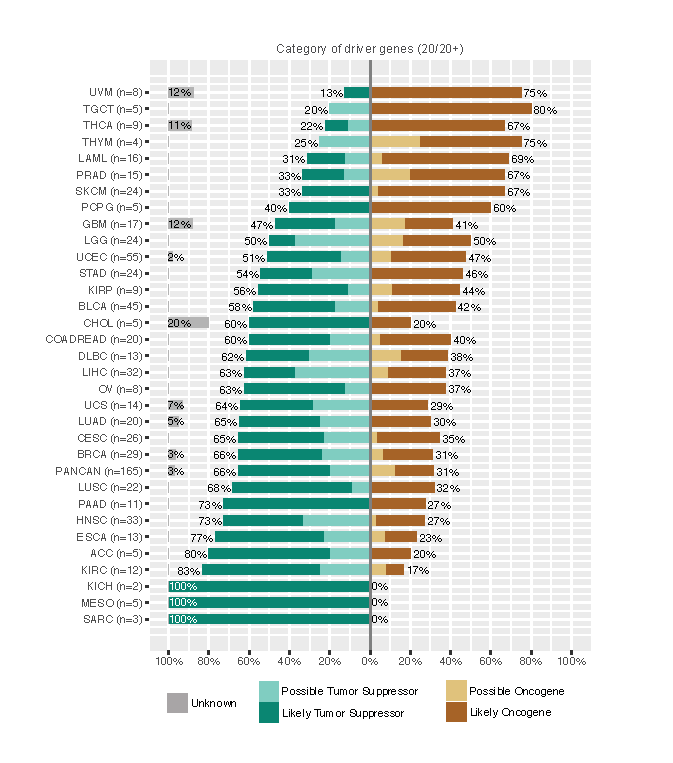
\includegraphics[width=0.9\linewidth]{figures/chapter7/og_tsg_balance.pdf}
  \caption[Balance of oncogenes and tumor suppressor genes.]{Balance of oncogenes and tumor suppressor genes. Percentage of consensus genes predicted as either oncogene (brown), tumor suppressor gene (green), or unknown (gray) by the 20/20+ algorithm, an improved version of the 20/20 rule. The 20/20+ algorithm uses a supervised-learning approach (random forests) and bases predictions on the mutational patterns observed within a gene. \q{Likely} and \q{Possible} statuses were determined at a threshold of 0.05 for q-value (Benjamini-Hochberg method) and p-value, respectively. Consensus genes were designated as \q{Unknown} if they did not meet these thresholds. N represents the number of significant genes in each cancer type.}
  \label{fig:og_tsg_balance}
\end{figure}

I clustered the different cancer types according to the consensus scores of their associated genes. Remarkably, some cancer types grouped according to their tissue of origin, such as LGG and GBM; while others according to their cell of origin. The most significant of the cell origin clusters spans all the squamous cancer types (BLCA, CESC, ESCA, HNSC and LUSC, (permutation test, adjusted p $<$ 0.01) and includes several transcription factors (ZNF750, NFE2L2 or KLF5), chromatin and histone modifiers (KMT2D, EP300, or NSD1), and various PI3K pathway genes (PIK3CA, PTEN or MAPK1). I found two additional significant clusters (permutation test, adjusted p $<$ 0.05) that group gynecological (UCS, CESC, UCEC, OV, and BRCA) as well as gastrointestinal cancers (COADREAD, PAAD, ESCA and STAD) (\autoref{fig:gene_discovery}A). 

Finally, I classified the consensus driver genes according to the cancer-related biological processes and pathways with which they were associated (\autoref{fig:gene_discovery}B). For most genes, the categories (excluding \q{other} and \q{other signaling}) clearly reflect known processes involved in carcinogenesis, as they are \q{transcription factor} (39 genes), \q{RTK signaling} (16) and \q{RNA abundance} (15), \q{protein homeostasis/ubiquitination} (15), \q{chromatin histone modifiers} (15), \q{genome integrity} (14), \q{chromatin other} (14) and, remarkably, \q{immune signaling} (10). The last group is of particular interest, given the connection between driver genes and immune response. In terms of cancer types, most have at least one cancer driver that belongs to either genome integrity (28 out of 33 cancer types) or the MAPK or PI3K signaling pathways (24 and 22 cancer types, respectively). Interestingly, the squamous cancer types were again grouped together when looking at which processes and pathways associated with their driver genes, having higher proportions of genes involved in chromatin histone modification as well as receptor-tyrosine kinase and immune signaling. 

\section{Driver mutation approach}

To maximize the coverage of our analysis I used 12 tools that look for three distinct hallmarks of \q{driverness}.  The collection was comprised of 8 mutation-level algorithms (SIFT \cite{RN9}, PolyPhen2 \cite{RN10}, MutationAssessor \cite{RN38}, transFIC \cite{RN53}, fathmm \cite{RN39}, CHASM \cite{RN29}, CanDrA \cite{RN36} and VEST \cite{RN30}), and 4 structure-based (HotSpot3D \cite{RN132}, HotMAPS \cite{RN60}, 3DHotSpots.org \cite{RN133} and e-Driver3D \cite{RN45}). In order to combine the predictions from the sequence-based approaches I used principal component analysis to develop a Combined Tool Adjusted Total (CTAT) scores for both, population-based and cancer-specific scores. Principal component analysis has been previously shown successful in a similar task of prioritizing germline mutations \cite{RN179}. I also combined the results from three-dimensional tools by adding the number of tools that predicted a specific position as belonging to a cancer-mutation cluster. Finally, to limit the number of false positives, I focused our analysis on the genes of our consensus driver list.

The CTAT score combines multiple individual tools that prioritize missense mutations. To normalize each score, I calculated the z-score by subtracting the mean score and then dividing by the standard deviation. I then performed principal component analysis (PCA) using ScikitLearn v0.18.0 and used the score along the first principal component as our CTAT score, representing the scalar projection onto the first eigenvector. Only missense mutations that had no missing values for each of the combined tools were used in generating the principal component analysis. I performed this procedure on two distinct categories of tools, \q{population-based} tools that distinguish damaging/pathogenic germline missense variants from common polymorphisms (SIFT, PolyPhen2, VEST, and MutationAssessor), and \q{cancer-focused} tools designed to distinguish somatic missense mutations that are drivers from passengers (CHASM, CanDrA, fathmm, and transFIC). To score the remaining missense mutations that did have a missing score, I imputed missing scores of the individual tool with the mean for the method. Imputation was only performed for the cancer-focused tools as the population-based tools had too many missing values.

To define the CTAT score thresholds, I used the maximum balanced accuracy when predicting OncoKB mutations \q{oncogenic} or \q{likely oncogenic}. This yielded a threshold of 1.2 for CTAT-population and 2.4 for CTAT-cancer. For the structural algorithms, I report a mutation as likely driver if at least 2 algorithms identify it within a cluster. Finally, I evaluated the performance of each CTAT score using mutations from OncoKB labeled as \q{likely oncogenic} or \q{oncogenic} as true-positives. 

\section{Discovery of driver mutations}

Not all mutations in a cancer driver gene have the same impact on its function \cite{RN183}. Their consequences frequently depend on which position within the protein is affected and what amino acid change is induced \cite{RN29}. Here, I sought to explore this topic across the entire PanCancer dataset, classifying 751,876 unique missense mutations by examining the 299 cancer driver genes that I identified, according to their predicted oncogenic effect. I combined the output of three different categories of tools into consensuses approaches: (I) tools that distinguish between benign and pathogenic mutations using sequence-based features (CTAT-population); (II) tools that distinguish between driver and passenger mutations using sequence-based features (CTAT-cancer); and (III) tools that discover statistically significant three-dimensional clusters of missense mutations (Structure-based); these identified 10,098 (1.3\% of the total missense mutations), 4,595 (0.6\%), and 1,469 (0.2\%) unique amino acid substitutions, respectively (\autoref{fig:driver_mutation}A). The differences in the number of predicted driver mutations for each approach are likely due to the design and requirements of the tools, i.e., dependence of structural clustering tools on available three-dimensional protein structures (either experimental or homology-based) yields fewer predicted driver mutations. Nevertheless, structural tools may provide additional molecular biological context for the identified mutations, which can be particularly relevant for variants of unknown significance (VUS) \cite{RN184}.

\begin{figure}
  \centering
  \makeatletter
  \let\@currsize\normalsize
  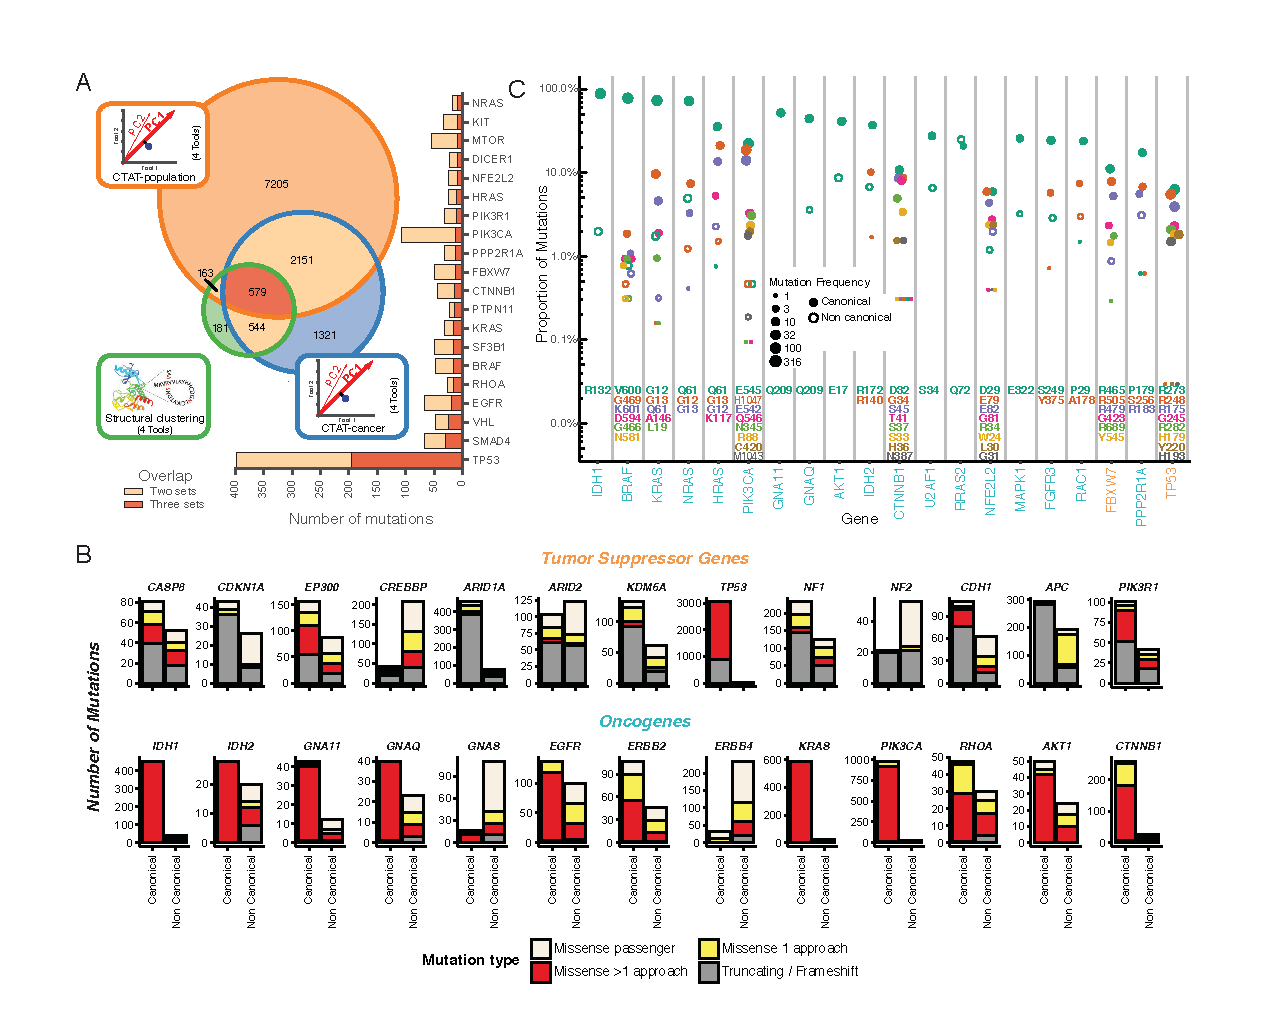
\includegraphics[width=\linewidth]{figures/chapter7/driver_mutation.pdf}
  \caption[Driver mutation discovery approaches, overview, overlap, and contrasts]{Driver mutation discovery approaches, overview, overlap, and contrasts: (A) Venn diagram indicates total number of mutations overlapping among three consensus approaches-CTAT-population, CTAT-cancer, and structural clustering. Adjacent bar chart indicates the top 20 genes sorted by 3-set intersecting mutation counts. (B) Driver gene discovery identified gene-tissue pairs (canonical genes) in tumor suppressors and oncogenes. However, some gene-tissue pairs were not identified in driver discovery (non-canonical). Mutation frequency from canonical and non-canonical cancer genes are displayed and divided among 4 mutation classes: truncation/frameshift mutations (grey); missense mutations uniquely identified by only one approach (yellow, see Panel A); missense mutations identified by multiple approaches (red, see Panel A); and missense passenger mutations not identified by any approach (off white). (C) Mutation percentage out of all missense and truncating/frameshift mutations within a gene is shown on the y-axis (log scale). Point size is log scaled and represents amino acid position frequency. The top 23 genes ordered by increasing mutational diversity (normalized entropy) and only the 9 most frequently mutated amino acid positions for each gene are shown.}
  \label{fig:driver_mutation}
\end{figure}

When benchmarked against OncoKB \cite{RN144}-a manually curated dataset of cancer mutations annotated according to likely oncogenic effect, cancer-focused algorithms had higher predictive value than algorithms that distinguished between benign and pathogenic mutations. In addition, the CTAT-cancer score outperformed all individual sequence-based approaches. 

Overall, there are 9,919 predicted cancer driver mutations in our cohort (3,437 unique mutations) identified by 2 or more approaches from CTAT-population, CTAT-cancer, or structural clustering. These mutations affect 5,782 tumor samples. I observed that these missense driver mutations represent a greater fraction of the total mutations in oncogenes than in tumor suppressors (\autoref{fig:driver_mutation}B). In this latter group, most mutations seem to be truncating or frameshift, a result in agreement with previous observations \cite{RN185}. Nevertheless, there are also tumor suppressor genes having high numbers of missense driver mutations, such as EP300, CREBBP, CASP8, PIK3R1 and TP53 (Figure 7.5B). An interesting example is CDH1, which is mostly affected by truncating or frameshift mutations in BRCA (75 out of 85 mutations), but mostly targeted by missense driver mutations in STAD (21 out of 25 mutations). This could suggest different roles for CDH1 in these two cancer types.

I was also intrigued by missense driver mutations detected in cancer types where the gene was not predicted to be a driver. This subset is particularly important for genotype-driven clinical trials \cite{RN186}. Overall, there are 1,719 of tissue-unmatched likely driver mutations (19\% of the total) in 1,431 patients (16\%) and there are 502 patients whose only predicted missense driver mutations affect genes not yet known to play a role in that cancer type. For example, I identified 28 patients with predicted EGFR driver mutations in cancer types where EGFR is not yet identified as a common driver gene, such as HNSC, STAD, LUSC, UCEC, ESCA and LIHC. In some extreme cases, such as ERBB4 or GNAS, these mutations actually represent the majority of predicted driver missense mutations in the gene (\autoref{fig:driver_mutation}B). Additionally, 2\% (10/457) of IDH1 missense events that occur at the amino acid position R132 are found in tissues not typically known to carry such mutations i.e. BLCA (n=2), BRCA (2), COADREAD (2), LUAD (2), PCPG (1), and THYM (1) (\autoref{fig:driver_mutation}C). Furthermore, I observed that RRAS2 Q72, a predicted oncogene in UCEC (n=5 samples) with strong homology to KRAS Q61 and HRAS Q61, was also mutated in cancer types in which it was not predicted to be an oncogene - UCS (n=1), LUSC (1), LUAD (1), PRAD (1), HNSC (1), and TCGT (1). Any analysis focusing only on common driver genes and mutations known in that cancer type would very likely miss presumed driver mutations for those patients. These results emphasize the advantage of PanCancer panels of driver mutations in order to maximize the coverage of driver-detection analyses.

\section{Value of structure-based analysis}

Results were compared to an independent dataset of 1,049 experimentally tested somatic mutations to validate our driver mutation predictions \cite{RN187}. Briefly, SNVs were introduced to two cancer cell lines, Ba/F3 and MCF10A, and were evaluated for their oncogenicity based on survival and growth. In total, 160 mutations from 19 genes were validated in this dataset. The percentage of functionally validated mutations increased from 60\% predicted with CTAT-population, to 61\% for those found by CTAT-cancer, and 78\% for Structure-based analysis (\autoref{fig:driver_mutation_examples}A). Among the 579 mutations predicted by all three approaches, 39 of the 46 that were tested (85\%) were also validated. Further, the sensitivity and specificity of identifying driver mutations annotated by OncoKB suggests performance is generalizable to a larger set of genes. These results support the value of the prediction algorithms used in our study and the advantage of combining multiple tools. Also, I would like to note that this approach only addresses true positive findings and represents a floor estimate for computational predictions.

\begin{figure}
  \centering
  \makeatletter
  \let\@currsize\normalsize
  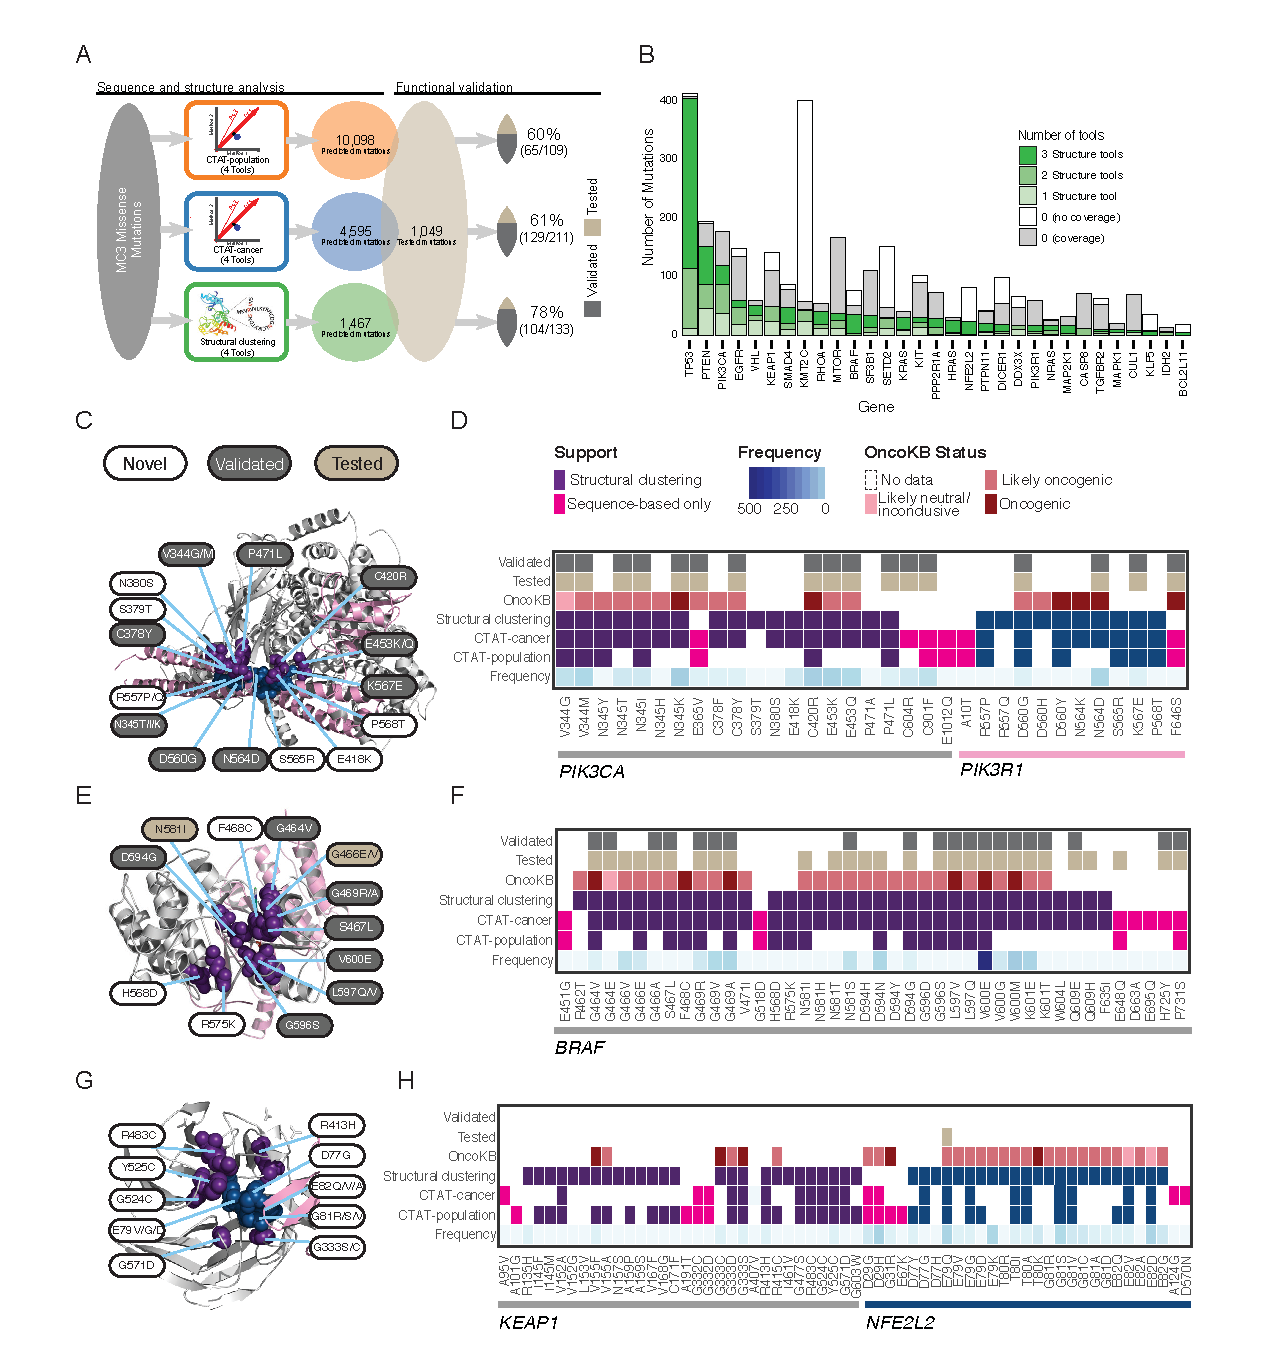
\includegraphics[width=\linewidth]{figures/chapter7/driver_mutation_examples.pdf}
  \caption[Driver mutation discovery and validation]{(Caption next page.)}
  \label{fig:driver_mutation_examples}
\end{figure}
\addtocounter{figure}{-1}
\begin{figure} [t!]
  \caption[(continued) Driver mutation discovery and validation]{(Figure: previous page) Driver mutation discovery and validation: (A) This schematic displays the steps taken to assess consensus among mutation-level predictions using sequence-based and structural clustering tools and comparing them to an orthogonal set of functionally validated mutations. From left to right: the grey box represents the missense mutations that were processed by 12 tools from 3 categories (population-based, cancer-focused, and structural clustering tools) and combined into three consensus approaches (CTAT-population, CTAT-cancer, and structural clustering). Finally, the total number and percentage of functionally validated/tested mutations is shown. (B) The number of mutations (y-axis) found by structural tools for each gene (x-axis) are shaded according to support by structural tools (green). Those mutations without support are distinguished by two categories, with (grey) and without (white) available protein structure.  Heatmaps (D, F, H) coupled with protein structure (C, E, G) are shown in panels for the proteins PIK3CA/PIK3R1 (PDB ID: 4OVU), BRAF (4MBJ), and KEAP1/NFE2L2 (3ZGC), respectively, and display whether a particular mutation was detected by sequence-based (CTAT-population or CTAT-cancer) or structure-based approaches (at least two structural tools). Purple/teal colors distinguish proteins (PIK3CA/PIK3R1 and KEAP1/NFE2L2 pairs) for mutations found by structure-based approaches, while pink boxes indicate mutations found only by sequence-based approach. Additionally, for each mutation, frequency (blue gradient), OncoKB status (red gradient), testing status (tan), and validation status (grey) are provided. All mutations found by structure-based approaches in each of the 3 genes are shown with a few additional mutations that are only found by sequence-based approaches. Key mutations are highlighted from the heatmaps and labeled with white, grey, and tan labels referring to novel, validated, and tested (not validated) mutations, respectively.}
\end{figure}

Structural-based mutations clustered on 66 proteins, including one cluster on KLF5, a gene not previously identified in PanCancer studies and ranked among the top 30 clusters by PanCancer mutation frequency (\autoref{fig:driver_mutation_examples}B). I sought to examine in more detail the predictions of the three approaches in various well-established cancer driver genes, such as PIK3CA/PIK3R1, BRAF, and KEAP1/NFE2L2 (\autoref{fig:driver_mutation_examples}C-4H). The interface between PIK3CA and PIK3R1 contains a cluster of mutations that were found by at least 2 of the approaches and includes both mutations that were validated and those not tested. D560G, N564D, and K567E are validated mutations that cluster closely to non-tested mutations R577P/Q, S565R, and P568T in PIK3R1. Similarly, PIK3CA contains validated mutations C378Y, V344G/M, N345T/I/K, P471L, C420R, and E418K clustering with non-tested mutations S379T, N380S, and E418K. These non-tested mutations are excellent candidates for further experimental validation due to their close proximity to known validated driver mutations as well as support from sequence-based approaches (\autoref{fig:driver_mutation_examples}C and \ref{fig:driver_mutation_examples}D). BRAF also contains clusters similar to this PIK3CA/PIK3R1 cluster, with a mixture of validated and novel mutations (\autoref{fig:driver_mutation_examples}E and \autoref{fig:driver_mutation_examples}F). 

Additionally, there are many genes that contain mutations found by all three approaches but that were not tested experimentally, including KEAP1, NFE2L2, RHOA, MTOR, MAP2K1, and VHL. Nevertheless, many of these driver mutations have orthogonal evidence from OncoKB. For example, the mutations G333D/S in KEAP1 have an OncoKB status of likely oncogenic and oncogenic, respectively (\autoref{fig:driver_mutation_examples}G and \ref{fig:driver_mutation_examples}H). There are also NFE2L2 mutations that cluster closely with the KEAP1 mutations along the protein-protein interface (D77, E82, G81, E79) and were not experimentally validated but have an OncoKB status of either likely-oncogenic or oncogenic. Other KEAP1 mutations in the same cluster found by all three approaches are R483C, Y525C, G524C, G571D, and R413H. However, none of these mutations were tested in our dataset, nor have evidence from OncoKB. Given their proximity to the validated KEAP1 sites and the bioinformatic evidence that I found, these mutations are ideal candidates for follow-up validation experiments. 

Overall, this analysis reinforces the notion that sequence-based approaches and structure-based approaches ought to be used in conjunction and tend to be complementary. For example, E365V, C604R, and C901F in PIK3CA, F646S in PIK3R1, and H725Y and P731S in BRAF were found by sequence-based approaches but not the structure-based approach and are experimentally validated (Figures \ref{fig:driver_mutation_examples}D and \ref{fig:driver_mutation_examples}F). Conversely, R462T in BRAF was only found through a structural approach and not sequence-based approaches and is annotated as likely oncogenic in OncoKB (Figures \ref{fig:driver_mutation_examples}F and \ref{fig:driver_mutation_examples}H). Finally, I note that, while looking at mutations detected by all 3 approaches provides high confident driver mutations, there may still be important driver mutations that were missed. 

\section{Conclusions}